\documentclass[12pt,letterpaper]{article}
\usepackage{graphicx,textcomp}
\usepackage{natbib}
\usepackage{setspace}
\usepackage{fullpage}
\usepackage{color}
\usepackage[reqno]{amsmath}
\usepackage{amsthm}
\usepackage{fancyvrb}
\usepackage{amssymb,enumerate}
\usepackage[all]{xy}
\usepackage{endnotes}
\usepackage{lscape}
\newtheorem{com}{Comment}
\usepackage{float}
\usepackage{hyperref}
\newtheorem{lem} {Lemma}
\newtheorem{prop}{Proposition}
\newtheorem{thm}{Theorem}
\newtheorem{defn}{Definition}
\newtheorem{cor}{Corollary}
\newtheorem{obs}{Observation}
\usepackage[compact]{titlesec}
\usepackage{dcolumn}
\usepackage{tikz}
\usetikzlibrary{arrows}
\usepackage{multirow}
\usepackage{xcolor}
\newcolumntype{.}{D{.}{.}{-1}}
\newcolumntype{d}[1]{D{.}{.}{#1}}
\definecolor{light-gray}{gray}{0.65}
\usepackage{url}
\usepackage{listings}
\usepackage{color}

\definecolor{codegreen}{rgb}{0,0.6,0}
\definecolor{codegray}{rgb}{0.5,0.5,0.5}
\definecolor{codepurple}{rgb}{0.58,0,0.82}
\definecolor{backcolour}{rgb}{0.95,0.95,0.92}

\lstdefinestyle{mystyle}{
	backgroundcolor=\color{backcolour},   
	commentstyle=\color{codegreen},
	keywordstyle=\color{magenta},
	numberstyle=\tiny\color{codegray},
	stringstyle=\color{codepurple},
	basicstyle=\footnotesize,
	breakatwhitespace=false,         
	breaklines=true,                 
	captionpos=b,                    
	keepspaces=true,                 
	numbers=left,                    
	numbersep=5pt,                  
	showspaces=false,                
	showstringspaces=false,
	showtabs=false,                  
	tabsize=2
}
\lstset{style=mystyle}
\newcommand{\Sref}[1]{Section~\ref{#1}}
\newtheorem{hyp}{Hypothesis}

\title{Problem Set 2}
\date{Due: October 15, 2023}
\author{Applied Stats/Quant Methods 1}

\begin{document}
	\maketitle
	\section*{Instructions}
\begin{itemize}
	\item Please show your work! You may lose points by simply writing in the answer. If the problem requires you to execute commands in \texttt{R}, please include the code you used to get your answers. Please also include the \texttt{.R} file that contains your code. If you are not sure if work needs to be shown for a particular problem, please ask.
	\item Your homework should be submitted electronically on GitHub.
	\item This problem set is due before 23:59 on Sunday October 15, 2023. No late assignments will be accepted.

\end{itemize}

	
	\vspace{.5cm}
	\section*{Question 1: Political Science}
		\vspace{.25cm}
	The following table was created using the data from a study run in a major Latin American city.\footnote{Fried, Lagunes, and Venkataramani (2010). ``Corruption and Inequality at the Crossroad: A Multimethod Study of Bribery and Discrimination in Latin America. \textit{Latin American Research Review}. 45 (1): 76-97.} As part of the experimental treatment in the study, one employee of the research team was chosen to make illegal left turns across traffic to draw the attention of the police officers on shift. Two employee drivers were upper class, two were lower class drivers, and the identity of the driver was randomly assigned per encounter. The researchers were interested in whether officers were more or less likely to solicit a bribe from drivers depending on their class (officers use phrases like, ``We can solve this the easy way'' to draw a bribe). The table below shows the resulting data.

\newpage
\begin{table}[h!]
	\centering
	\begin{tabular}{l | c c c }
		& Not Stopped & Bribe requested & Stopped/given warning \\
		\\[-1.8ex] 
		\hline \\[-1.8ex]
		Upper class & 14 & 6 & 7 \\
		Lower class & 7 & 7 & 1 \\
		\hline
	\end{tabular}
\end{table}

\begin{enumerate}
	
	\item [(a)]
	Calculate the $\chi^2$ test statistic by hand/manually (even better if you can do "by hand" in \texttt{R}).\\
	\vspace{7cm}
\begin{lstlisting}
# Just getting the table, in R studio t be able to work the rest

data <- matrix(c(14, 7, 6, 7, 7, 1), ncol=3)
rownames(data) <- c('Upper Class', 'Lower Class')
colnames(data) <- c('Not Stopped', 'Bribe Requested', 'Stopped/Given warning')
data <- as.table(data)data
# Doing the sums in order to get to the expected frequencies
sum_of_rows <- rowSums(data)
sum_of_cols <- colSums(data)
table_sum <- addmargins(data, FUN = sum)
data
gp <- ggplot(aes, x=)
# I tried to get the addmargins going but it printed nothing.
# So I had to do all this middle bits to be able to get my totals added to my table
class(data)
str(data)
addmargins(data)
# the next part is to calculate the expected frequencies
expDat <- data.frame() 
for (i in 1:3) \{  
expDat[i, 1] <- (sum(data[i,]) * sum
(data[, 1])) / sum(data) 
expDat[i, 2] <- (sum(data[i,]) * sum
(data[, 2])) / sum(data)  
expDat[i, 3] <- (sum(data[i,]) * sum
(data[, 3])) / sum(data)
}
expDat
#when running expDat there was an error message but it still gave me the values I was looking for 
# the values found are the expected frequencies
\end{lstlisting}		

\begin{table}[h!]
 \centering
\begin{tabular}{l | c c c c}
   & Not Stopped & Bribe requested & Stopped/given warning & Totals \\
   \\[-1.8ex]
   \hline\\[-1.8ex]
   Upper class & 14 & 6 & 7 & 27 \\
   Lower class & 7 & 7 & 1 & 15 \\
   Totals & 21 & 13 & 8 & 42 \\
   \hline
   \end{tabular}
\end{table}

\begin{table}[h!]
	\centering
	\begin{tabular}{l | c c c }
		& Not Stopped & Bribe requested & Stopped/given warning \\
		\\[-1.8ex] 
		\hline \\[-1.8ex]
		Upper class & 13.5 & 8.35 & 5.14 \\
		Lower class & 7.49 & 4.64 & 2.85 \\
		\hline
	\end{tabular}
\end{table}



\begin{lstlisting}
# Calculating chi square without the function, like a formula 
ChiSqr <- sum((data - expDat)^2/expDat)
ChiSqr
# the output was 3.79
# to confirm that my "formula" works the same as the function
xisq <- chisq.test(data)
xisq
# out put X-squared = 3.7912, df = 2, p-value = 0.1502
\end{lstlisting}

	\item [(b)]
	Now calculate the p-value from the test statistic you just created (in \texttt{R}).\footnote{Remember frequency should be $>$ 5 for all cells, but let's calculate the p-value here anyway.}  What do you conclude if $\alpha = 0.1$?\\
	
\begin{lstlisting}
# Calculating degree of freedom
# df <- (nrow - 1)(ncol - 1) # how do i do this?
# df <- (2-1)(3-1)
# df <- (1)*(2)
# df <- 2
# this was kind of calculating by hand
# and now comes the formula in R
nrow <- 2
ncol <- 3
df <- (nrow-1) * (ncol-1)
df
# Calculating pvalue
p_value <- pchisq(3.79, df=2, lower.tail = FALSE)p_value
# output 0.1503
	\end{lstlisting}
	
\begin{verbatim}
	If the p value is bigger than alpha then we can not reject the null hypothesis.
	 The null hypothesis is that there are no differences in the frequency of 
	 asking for a bribe between drivers of different socio-economic classes. 
	 The alternative hypothesis is that there are differences in the frequency 
	 bribes are requested depending on drivers socio-economic class. 
	 In this case alpha is 0.1 and p is 0.15 so p>alpha and we can't reject the H0.
\end{verbatim}
	
	\newpage
	\item [(c)] Calculate the standardized residuals for each cell and put them in the table below.
	\vspace{1cm}
	
	\begin{math}
		\frac{fob - fex}{\sqrt{fe(1 - rowprop)(1 - collumnprop)}}
	\end{math}	
	\vspace{1cm}
	\begin{equation}
		14 - 13.5 /\sqrt{13.5 (1 - (27/42))(1 - (21/42))}
	\end{equation}
	\begin{equation}
		7 - 7.49 /\sqrt{7.49 (1 - (15/42))(1 - (21/42))}
    \end{equation}	
    \begin{equation}
    	6 - 8.35 /\sqrt{8.35 (1 - (27/42))(1 - (13/42))}
    \end{equation}	
    	\begin{equation}
    	7 - 4.64 /\sqrt{4.64 (1 - (15/42))(1 - (13/42))}
    \end{equation}	
    \begin{equation}
    	7 - 5.14 /\sqrt{5.14 (1 - (27/42))(1 - (8/42))}
    \end{equation}
    \begin{equation}
    	1 - 2.85 /\sqrt{2.85 (1 - (15/42))(1 - (8/42))}
    \end{equation}		
	\begin{table}[h]
		\centering
		\begin{tabular}{l | c c c }
			& Not Stopped & Bribe requested & Stopped/given warning \\
			\\[-1.8ex] 
			\hline \\[-1.8ex]
			Upper class  & 0.32 & -1.62 & 1.52 \\
			\\
			Lower class & -0.31 & 1.62  & -1.51  \\
			
		\end{tabular}
	\end{table}
	
	
	\vspace{7cm}
	\item [(d)] How might the standardized residuals help you interpret the results?  
\begin{verbatim}
The standardised residuals are symmetrical , suggesting a normal distribution and
a non linear relationship between the two variables.
\end{verbatim}
\end{enumerate}
\newpage

\section*{Question 2: Economics}
Chattopadhyay and Duflo were interested in whether women promote different policies than men.\footnote{Chattopadhyay and Duflo. (2004). ``Women as Policy Makers: Evidence from a Randomized Policy Experiment in India. \textit{Econometrica}. 72 (5), 1409-1443.} Answering this question with observational data is pretty difficult due to potential confounding problems (e.g. the districts that choose female politicians are likely to systematically differ in other aspects too). Hence, they exploit a randomized policy experiment in India, where since the mid-1990s, $\frac{1}{3}$ of village council heads have been randomly reserved for women. A subset of the data from West Bengal can be found at the following link: \url{https://raw.githubusercontent.com/kosukeimai/qss/master/PREDICTION/women.csv}\\

\noindent Each observation in the data set represents a village and there are two villages associated with one GP (i.e. a level of government is called "GP"). Figure~\ref{fig:women_desc} below shows the names and descriptions of the variables in the dataset. The authors hypothesize that female politicians are more likely to support policies female voters want. Researchers found that more women complain about the quality of drinking water than men. You need to estimate the effect of the reservation policy on the number of new or repaired drinking water facilities in the villages.
\vspace{.5cm}
\graphicspath{{./StatsI_Fall2023/}}
\begin{figure}[h!]
	\caption{\footnotesize{Names and description of variables from Chattopadhyay and Duflo (2004).}}
	\vspace{.5cm}
	\centering
	\label{fig:women_desc}
	\includegraphics[width=1.1\textwidth]{women_desc}
\end{figure}		

\newpage
\begin{enumerate}
	\item [(a)] State a null and alternative (two-tailed) hypothesis. 
	
\begin{verbatim}
	The null hypothesis is that the reserve policy has no influence on the number of
	new or repaired water facilitiesin the villages and the alternative hypothesis
	is that the reserve policy affects the number of repaired or new water facilities
    in the villages.
\end{verbatim}
	\vspace{6cm}
	\item [(b)] Run a bivariate regression to test this hypothesis in \texttt{R} (include your code!).
\begin{lstlisting}
# reading the data set to visualise it and so R knows what I will be talking
#about
urlfile="https://raw.githubusercontent.com/kosukeimai/qss/master/PREDICTION/women.csv"
datfra <-read_csv(url(urlfile))
spec(datfra)
head(datfra)
print(datfra)
# It kept printing only parts of the data and I was afraid that R wouldn't read it all when plotting
# so I determined what to print
print(datfra, n=400)
# then to run the regression. 
Y1 <- "reserved"
X1 <- "water"
model1 <- lm(water~reserved, data = datfra)
model1
# output 
# Call:lm(formula = water ~ reserved, data = datfra)
# Coefficients:
# (Intercept)     reserved
#      14.738        9.252  
summary(model1)
# output
# Call:lm(formula = water ~ reserved, data = datfra)
# Residuals:
#    Min       1Q    Median      3Q     Max 
#  -23.991   -14.738  -7.865   2.262   316.009
# Coefficients:          
#                    Estimate    Std. Error   t value      Pr(>|t|) 
#   (Intercept)    14.738       2.286          6.446       4.22e-10 ***
#    reserved       9.252        3.948          2.344       0.0197 *
# Residual standard error: 33.45 on 320 degrees of freedom
# Multiple R-squared:  0.01688,	Adjusted R-squared:  0.0138 
# F-statistic: 5.493 on 1 and 320 DF,  p-value: 0.0197
\end{lstlisting}

\begin{lstlisting}
# I plotted the variables and calculated the correlation to help me visualise things
plot(x=datfra$reserved, y=datfra$water, xlim=c(0,2), ylim=c(0,320))
cor.test(datfra$reserved, datfra$water)
# output
# Pearson's product-moment correlation
# data:  datfra$reserved and datfra$water
# t = 2.3437, df = 320, p-value = 0.0197
# alternative hypothesis: true correlation is not equal to 
# 095 percent confidence interval: 0.02090616 0.23585751sample estimates:      
# cor 0.1299079 
\end{lstlisting}	
	
\graphicspath{{./StatsI_Fall2023/}}
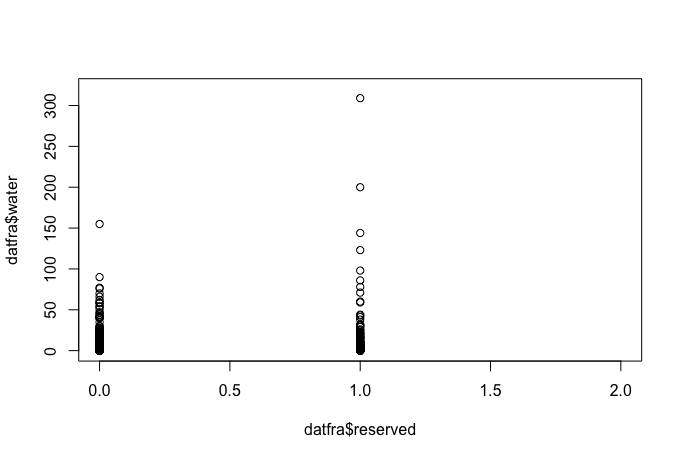
\includegraphics[width=15cm]{Rplot_reserved_water}
\begin{verbatim}
with  p-value of 0.019, if we assume an alpha of 0.05, we have sufficient
evidence to reject the null hypothesis. However with a correlation coefficient
of 0.129 we can say that there is a weak correlation between the two variables,
since a strong correlation would be considered to have a correlation coefficient 
close to 1 for a positive correlation and close to -1 for a negative correlation. 
\end{verbatim}
	\vspace{6cm}
	\item [(c)] Interpret the coefficient estimate for reservation policy. 
	
\begin{verbatim}
	The coefficiet estimates tell us; first, that according to the intercept = 14.73,
	the average of water facilities (new or repaired) in the villages if there were 
	no reserved places for women leaders. The slope is 9.25 meaning that for 
	every increase of 1 reserved place the number of water facilities increases
	by 9.25.
\end{verbatim}	
\end{enumerate}

\end{document}
